\section{Benchmarkting}

Nesta secção falar-se-á dos resultados obtidos e analisar-se-ão os mesmos. Vamos começar por apresentar a validação do classificador onde não se utilizaram janelas para remover o ruido e posteriormente serão apresentadas todas as janelas testadas com os respetivos filtros.\newline
É de sublinhar que cada uma das implementações testada foi corrida 9 vezes após a sua otimização, este processo é essencial uma vez que ao utilizarmos o método do gradiente estocástico inserimos um componente aleatório na convergência, ou seja é necessário realizar vários testes para garantir que este método não prejudica os resultados obtidos calibrando mal os pesos ou não permitindo a melhor calibração dos mesmos que se obteria por outros métodos mais precisos embora mais demorados.
Quanto á otimização levada a cabo em cada uma das versões do logistic classifier convêm referir algumas regras básicas que foram seguidas neste trabalho.
\begin{itemize}

	\item Devemos observar a variação do erro pós refinamento dos pesos para garantir que este não é errático o que indica que o learning rate é muito grande\cite{ref4}.
	\item É necessário verificar se o erro se torna estático durante algumas dezenas de epochs, este estaticismo revela que o número de epochs é demasiado elevado ou que o learning rate é demasiado baixo, no entanto caso este learning rate após dezenas de epochs em que a variação do erro tende a diminuir se tornar errático devemos truncar as epochs  até ao momento em que o erro se torna errático e repetir o refinamento dos pesos a partir dese ponto com um learning rate mais baixo\cite{ref4}.\hfill\newline
	\item Convêm saber que, por norma, o decréscimo do learning rate tende a situar-se algures entre 1/4 e 3/4 do valor anterior, verificando-se mais comummente o valor de 1/2, sendo este depois ajustado baseado nos resultados da progressão dos erros\cite{ref7}.
\end{itemize}


\subsection{Validação do Classificador}

Esta implementação trata-se do classificador genérico, este não faz uso nem de janelas deslizantes nem de filtros, em vez disso processa todas as imagens na sua totalidade. A progressão dos valores de erro e a tabela de confusão obtida após a otimização dos pesos do mesmo pode ser vista em baixo.

\begin{figure}[H]

  \centering
  \captionsetup{justification=centering}

  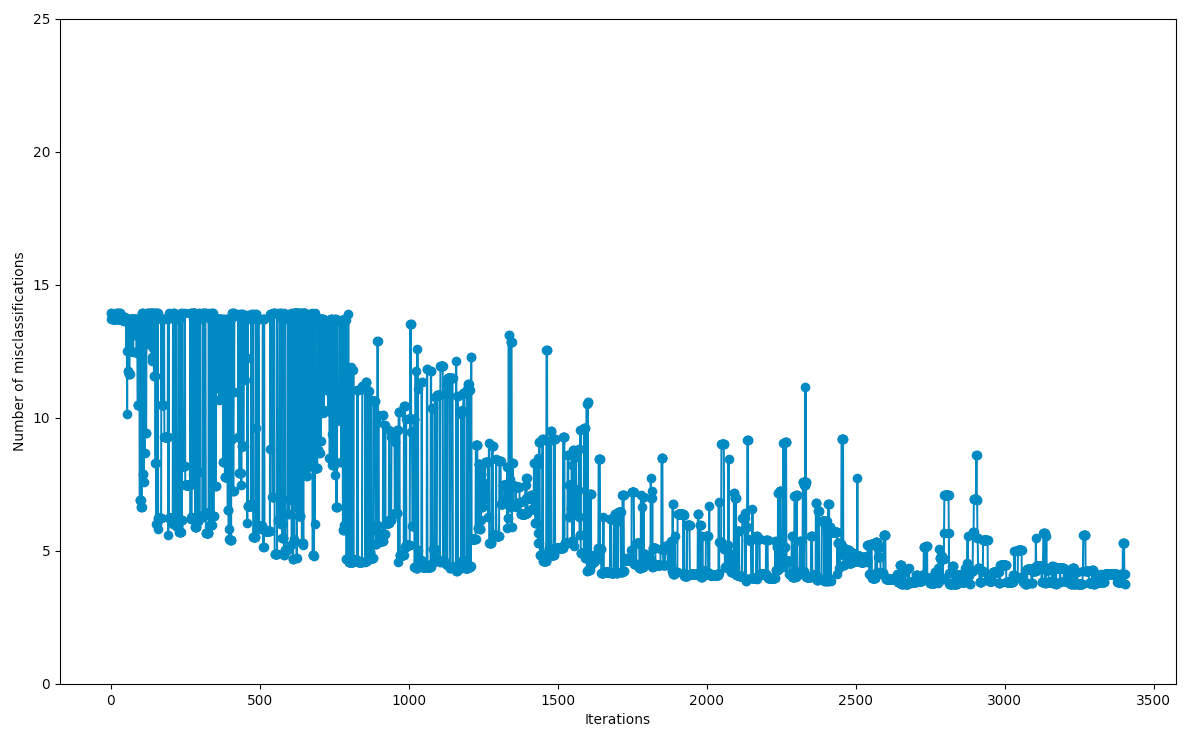
\includegraphics[width = 0.7\textwidth]{erros2_v1.png}
  
  \caption {Progressão dos erros da versão de validação}
\end{figure}

\begin{figure}[H]

  \centering
  \captionsetup{justification=centering}

  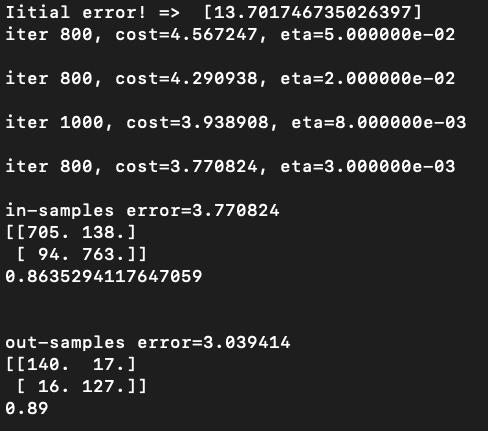
\includegraphics[width = 0.6\textwidth]{confusao2_v1.png}
  
  \caption {Tabelas de confusão da versão de validação}
\end{figure}


Como podemos ver na tabela de confusão do out-sample temos 300 imagens das quais 46 foram mal classificadas o que nos deixa com uma taxa de sucesso de 89\%. Através da representação dos erros no gráfico podemos verificar que a os erros tendem a estabilizar perto do valor 3,7 uma vez que a curva de otimização se comporta de tal forma que tende a estabilizar e a minimizar os ganhos em termos de taxa de sucesso face ao treino empregue após atingir este valor. Esta versão demora cerca de 23 minutos e 48 segundos a executar.\hfill\newline
Note-se também que existe underfitting dos dados de treino face aos dados de teste, indicando que caso o vetor de pesos seja usado para classificar um dataset de 3 e 8 maior os resultados não deverão desviar-se muito dos obtidos em cima embora possam piorar uma vez que o underfitting mostra que o modelo não se adaptou muito bem aos dados de treino.\newline
No presente momento podemos dizer que o dataset não é linearmente separável na sua totalidade uma vez que não conseguimos separar 11\% das imagens do out-sample.
 



\subsection{Análise dos Poolings Clássicos}

Nesta secção será abordada a utilização dos poolings denominados clássicos para avaliar os benefícios que estes fornecem á taxa de sucesso de previsão e aos tempos de execução do treino e teste do modelo. Estes serão apresentados na tabela abaixo pela mesma ordem em que foram implementados juntamente com os respetivos resultados\footnote{Para cada um dos poolings procedeu-se também a uma otimização dos parâmetros de learning rate e número de epochs.}. Note-se que, para cada combinação de janela e filtro de pooling, se realizaram 9 execuções do código e que o resultado apresentado é o melhor valor obtido dessas 9 execuções. Note-se também que as in-samples e out-samples serão referenciadas como $in$ e $out$ e que os seus valores estão em percentagem, e que os valores no campo time se encontram em minutos e segundos.

\begin{table}[h]
	\resizebox{\textwidth}{!}{ %
	\begin{tabular}{||c|c|c|c|c|c|c|c|c|c|c|c|c||}
	\hline
	\multirow{2}{*}{\backslashbox{Filtro}{Janela}}  & \multicolumn{3}{|c|}{2x2} & \multicolumn{3}{|c|}{2x3} & \multicolumn{3}{|c|}{3x2} & \multicolumn{3}{|c|}{3x3} \\ \cline{2-13}
	 &  \textbf{in}(\%) & \textbf{out}(\%) & \textbf{time}  & \textbf{in}(\%) & \textbf{out}(\%) & \textbf{time} &  \textbf{in}(\%) & \textbf{out}(\%) & \textbf{time} &  \textbf{in}(\%) & \textbf{out}(\%) & \textbf{time} \\ \hline


	Max           & 75,00 & 75,00 & 17:00 & 67,40 & 69,00 & 11:38 & 66,94 & 69,00 & 8:48 & 88,00 & 88,67 & 6:32 \\ \hline
	Min           & 86,00 & 89,30 & 16:09 & 88,18 & 90,00 & 9:11 & 87,71 & 90,00 & 11:40 & 89,88 & 90,33 & 6:34 \\ \hline
	Average       & 85,70 & 85,67 & 17:46 & 84,18 & 86,67 & 9:52 & 78,65 & 83,33 & 12:52 & 83,06 & 82,33 & 3:04 \\ \hline
	Max Centered  & 88,60 & 88,30 & 21:02 & 88,06 & 90,00 & 13:58 & 88,00 & 90,00 & 8:32 & 86,29 & 89,00 & 6:51 \\ \hline

	\end{tabular}%
	}
\end{table}


\begin{table}[h]
	\centering
	\resizebox{0.6\textwidth}{!}{ %
	\begin{tabular}{||c||c|c|c|c|c|c|c|c|c|c|c|c||}
	\hline
	\multirow{2}{*}{Validação do Classificador}    & in-sample(\%) & out-sample(\%) & time  \\\cline{2-4}
	& 86,35 & 89,00 & 23:48 \\\hline

	\end{tabular}%
	}
\end{table}


Nesta tabela temos vários resultados que se mostram melhores que os obtidos aquando da validação do classificador, sendo que esses resultados são fruto da conjugação dos filtros "Min" e "Max Centered" com as várias janelas utilizadas. Por outro lado o filtro "Max" teve maus resultados conjugado com todas as janelas exceto a 3x3. \newline
No caso do filtro Min podemos observar que á medida que aumentamos as dimensões da janela os resultados tendem a melhorar e o underfitting do modelo tende a diminuir, sendo o seu menor valor 0.45\% no caso da janela 3x3. O modelo resultante da conjugação do fitro Min com a janela 3x3 e stride 2 nas dimensões x e y foi aquele que produziu o melhor resultado uma vez que apresenta juntamente com a melhor taxa de sucesso nas previsões, a menor taxa de underfitting e o melhor tempo demorando apenas 6 minutos e 34 segundos a executar.\newline
É também importante realçar que comparando os resultados obtidos das conjugações dos diferentes filtros empregues com as janelas 2x3 e 3x2 se verifica que a janela 2x3 é em geral melhor para prever os dados por possuir menor underfitting, isto é as imagens do dataset são melhor classificadas caso se use uma janela que possua dimensões em $y$ maiores do que em $x$.



\subsection{Análise dos Poolings Exóticos}

Nesta secção será analisada a utilização dos poolings exóticos implementados e explicados na secção anterior. Mais uma vez executaram-se 9 vezes cada combinação de janela e filtro e apenas o melhor resultado de cada combinação é apresentado. Adicionalmente sublinha-se que as in-samples e out-samples encontram-se na tabela referenciadas como $in$ e $out$ e os seus valores encontram-se em percentagem. Uma vez que os nomes dos filtros exóticos são extensos utilizar-se-ão as iniciais de cada um e estes serão apresentados na tabela pela ordem de apresentação dos mesmos na subsecção~\ref{subsec:poolingExotico}. 


\begin{table}[h]
	\resizebox{\textwidth}{!}{ %
	\begin{tabular}{||c|c|c|c|c|c|c|c|c|c|c|c|c||}
	\hline
	\multirow{2}{*}{\backslashbox{Filtro}{Janela}}  & \multicolumn{3}{|c|}{2x2} & \multicolumn{3}{|c|}{2x3} & \multicolumn{3}{|c|}{3x2} & \multicolumn{3}{|c|}{3x3} \\ \cline{2-13}
	 &  \textbf{in}(\%) & \textbf{out}(\%) & \textbf{time}  & \textbf{in}(\%) & \textbf{out}(\%) & \textbf{time} &  \textbf{in}(\%) & \textbf{out}(\%) & \textbf{time} &  \textbf{in}(\%) & \textbf{out}(\%) & \textbf{time} \\ \hline

 DVAP & 83,65 & 87,00 & 13:03 & 84,18 & 87,00 & 6:24 & 84,18 & 87,00 & 6:35 & 81,06 & 82,00 & 5:33 \\ \hline
DVMCP & 89,24 & 87,67 & 15:43 & 84,29 & 86,67 & 6:40 & 88,76 & 90,00 & 6:57 & 86,59 & 90,33 & 6:54 \\ \hline
 DVMP & 86,35 & 90,33 & 20:33 & 88,67 & 83,41 & 8:37 & 85,82 & 89,33 & 8:58 & 87,53 & 89,00 & 4:26 \\ \hline
DVMAP & 86,12 & 89,67 & 21:33 & 86,12 & 87,67 & 10:07 & 85,76 & 88,33 & 8:30 & 83,88 & 85,00 & 4:42 \\ \hline

	\end{tabular}%
	}
\end{table}

\begin{table}[h]
	\centering
	\resizebox{0.6\textwidth}{!}{ %
	\begin{tabular}{||c||c|c|c|c|c|c|c|c|c|c|c|c||}
	\hline
	\multirow{2}{*}{Validação do Classificador}    & in-sample(\%) & out-sample(\%) & time  \\\cline{2-4}
	& 86,35 & 89,00 & 23:48 \\\hline

	\end{tabular}%
	}
\end{table}


No geral os resultados obtidos com a aplicação dos poolings exóticos são inferiores aos obtidos com poolings clássicos. No entanto, existem 2 resultados que superam os anteriormente vistos, nomeadamente a conjugação do filtro Diagonal and Vertical Max Pooling com a janela 2x2 e do filtro Diagonal and Vertical Max Centered Pooling com a janela 3x3. Embora ambos tenham um resultado de out-sample igual, o segundo pooling referido oferece 2 vantagens face ao primeiro. Além de possuir um underfitting ligeiramente inferior é pelo menos três vezes mais rápido a executar fazendo deste a escolha obvia como o melhor modelo dos dois.\newline
\hfill\newline
Comparando todos os resultados obtidos durante os testes podemos concluir que o melhor modelo se trata daquele resultante da aplicação do filtro "Min" á janela 3x3 por se tratar do mais rápido com menor underfitting e melhor valor preditivo. Adicionalmente podemos concluir que cerca de 9-10\% desta base de dados não é linearmente separável, totalizando cerca de 27-30 imagens do dataset de treino as quais o nosso melhor modelo não consegue separar. 

Adicionalmente procurou-se saber qual a janela minima a utilizar para se verificar uma perda total de informação útil para além de ruido. Verificou-se que a perda de informação útil se começa a dar a partir da janela de dimensões 6x5 com strides 5 em x e 4 em y. \newline
O cenário onde se verificou a perda total de informação útil deu-se quando se utilizou uma janela de tamanho 10x9 com strides 9 em x e 8 em y, resultando em imagens de 9 pixeis quase impossiveis de se distinguirem como se pode verificar na matriz de confusão obtida.

\begin{figure}[H]
	
\captionsetup{justification=centering}
  \begin{subfigure}{.5\textwidth}
  \centering
  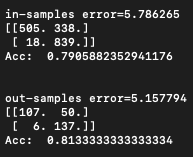
\includegraphics[width = 0.6\textwidth]{first_result.png}
  \caption {Tabelas de confusão da janela 6x5}
  \end{subfigure}
  \begin{subfigure}{.5\textwidth}
  \centering
  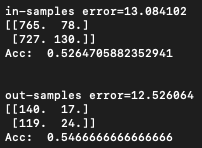
\includegraphics[width = 0.67\textwidth]{worst_result.png}
  \caption {Tabelas de confusão da janela 10x9}
  \end{subfigure}
\end{figure}


















